% Options for packages loaded elsewhere
\PassOptionsToPackage{unicode}{hyperref}
\PassOptionsToPackage{hyphens}{url}
%
\documentclass[
  man]{apa6}
\usepackage{amsmath,amssymb}
\usepackage{lmodern}
\usepackage{iftex}
\ifPDFTeX
  \usepackage[T1]{fontenc}
  \usepackage[utf8]{inputenc}
  \usepackage{textcomp} % provide euro and other symbols
\else % if luatex or xetex
  \usepackage{unicode-math}
  \defaultfontfeatures{Scale=MatchLowercase}
  \defaultfontfeatures[\rmfamily]{Ligatures=TeX,Scale=1}
\fi
% Use upquote if available, for straight quotes in verbatim environments
\IfFileExists{upquote.sty}{\usepackage{upquote}}{}
\IfFileExists{microtype.sty}{% use microtype if available
  \usepackage[]{microtype}
  \UseMicrotypeSet[protrusion]{basicmath} % disable protrusion for tt fonts
}{}
\makeatletter
\@ifundefined{KOMAClassName}{% if non-KOMA class
  \IfFileExists{parskip.sty}{%
    \usepackage{parskip}
  }{% else
    \setlength{\parindent}{0pt}
    \setlength{\parskip}{6pt plus 2pt minus 1pt}}
}{% if KOMA class
  \KOMAoptions{parskip=half}}
\makeatother
\usepackage{xcolor}
\IfFileExists{xurl.sty}{\usepackage{xurl}}{} % add URL line breaks if available
\IfFileExists{bookmark.sty}{\usepackage{bookmark}}{\usepackage{hyperref}}
\hypersetup{
  pdftitle={Developmental consistency in children's drawings of object categories},
  pdfauthor={Bria Long1, Ying Wang2, Stella Christie2, Michael C. Frank1, \& Judith E. Fan3},
  pdflang={en-EN},
  pdfkeywords={children's drawings, visual production, tracing, object recognition, visuomotor control},
  hidelinks,
  pdfcreator={LaTeX via pandoc}}
\urlstyle{same} % disable monospaced font for URLs
\usepackage{graphicx}
\makeatletter
\def\maxwidth{\ifdim\Gin@nat@width>\linewidth\linewidth\else\Gin@nat@width\fi}
\def\maxheight{\ifdim\Gin@nat@height>\textheight\textheight\else\Gin@nat@height\fi}
\makeatother
% Scale images if necessary, so that they will not overflow the page
% margins by default, and it is still possible to overwrite the defaults
% using explicit options in \includegraphics[width, height, ...]{}
\setkeys{Gin}{width=\maxwidth,height=\maxheight,keepaspectratio}
% Set default figure placement to htbp
\makeatletter
\def\fps@figure{htbp}
\makeatother
\setlength{\emergencystretch}{3em} % prevent overfull lines
\providecommand{\tightlist}{%
  \setlength{\itemsep}{0pt}\setlength{\parskip}{0pt}}
\setcounter{secnumdepth}{-\maxdimen} % remove section numbering
% Make \paragraph and \subparagraph free-standing
\ifx\paragraph\undefined\else
  \let\oldparagraph\paragraph
  \renewcommand{\paragraph}[1]{\oldparagraph{#1}\mbox{}}
\fi
\ifx\subparagraph\undefined\else
  \let\oldsubparagraph\subparagraph
  \renewcommand{\subparagraph}[1]{\oldsubparagraph{#1}\mbox{}}
\fi
\newlength{\cslhangindent}
\setlength{\cslhangindent}{1.5em}
\newlength{\csllabelwidth}
\setlength{\csllabelwidth}{3em}
\newlength{\cslentryspacingunit} % times entry-spacing
\setlength{\cslentryspacingunit}{\parskip}
\newenvironment{CSLReferences}[2] % #1 hanging-ident, #2 entry spacing
 {% don't indent paragraphs
  \setlength{\parindent}{0pt}
  % turn on hanging indent if param 1 is 1
  \ifodd #1
  \let\oldpar\par
  \def\par{\hangindent=\cslhangindent\oldpar}
  \fi
  % set entry spacing
  \setlength{\parskip}{#2\cslentryspacingunit}
 }%
 {}
\usepackage{calc}
\newcommand{\CSLBlock}[1]{#1\hfill\break}
\newcommand{\CSLLeftMargin}[1]{\parbox[t]{\csllabelwidth}{#1}}
\newcommand{\CSLRightInline}[1]{\parbox[t]{\linewidth - \csllabelwidth}{#1}\break}
\newcommand{\CSLIndent}[1]{\hspace{\cslhangindent}#1}
\ifLuaTeX
\usepackage[bidi=basic]{babel}
\else
\usepackage[bidi=default]{babel}
\fi
\babelprovide[main,import]{english}
% get rid of language-specific shorthands (see #6817):
\let\LanguageShortHands\languageshorthands
\def\languageshorthands#1{}
% Manuscript styling
\usepackage{upgreek}
\captionsetup{font=singlespacing,justification=justified}

% Table formatting
\usepackage{longtable}
\usepackage{lscape}
% \usepackage[counterclockwise]{rotating}   % Landscape page setup for large tables
\usepackage{multirow}		% Table styling
\usepackage{tabularx}		% Control Column width
\usepackage[flushleft]{threeparttable}	% Allows for three part tables with a specified notes section
\usepackage{threeparttablex}            % Lets threeparttable work with longtable

% Create new environments so endfloat can handle them
% \newenvironment{ltable}
%   {\begin{landscape}\centering\begin{threeparttable}}
%   {\end{threeparttable}\end{landscape}}
\newenvironment{lltable}{\begin{landscape}\centering\begin{ThreePartTable}}{\end{ThreePartTable}\end{landscape}}

% Enables adjusting longtable caption width to table width
% Solution found at http://golatex.de/longtable-mit-caption-so-breit-wie-die-tabelle-t15767.html
\makeatletter
\newcommand\LastLTentrywidth{1em}
\newlength\longtablewidth
\setlength{\longtablewidth}{1in}
\newcommand{\getlongtablewidth}{\begingroup \ifcsname LT@\roman{LT@tables}\endcsname \global\longtablewidth=0pt \renewcommand{\LT@entry}[2]{\global\advance\longtablewidth by ##2\relax\gdef\LastLTentrywidth{##2}}\@nameuse{LT@\roman{LT@tables}} \fi \endgroup}

% \setlength{\parindent}{0.5in}
% \setlength{\parskip}{0pt plus 0pt minus 0pt}

% Overwrite redefinition of paragraph and subparagraph by the default LaTeX template
% See https://github.com/crsh/papaja/issues/292
\makeatletter
\renewcommand{\paragraph}{\@startsection{paragraph}{4}{\parindent}%
  {0\baselineskip \@plus 0.2ex \@minus 0.2ex}%
  {-1em}%
  {\normalfont\normalsize\bfseries\itshape\typesectitle}}

\renewcommand{\subparagraph}[1]{\@startsection{subparagraph}{5}{1em}%
  {0\baselineskip \@plus 0.2ex \@minus 0.2ex}%
  {-\z@\relax}%
  {\normalfont\normalsize\itshape\hspace{\parindent}{#1}\textit{\addperi}}{\relax}}
\makeatother

% \usepackage{etoolbox}
\makeatletter
\patchcmd{\HyOrg@maketitle}
  {\section{\normalfont\normalsize\abstractname}}
  {\section*{\normalfont\normalsize\abstractname}}
  {}{\typeout{Failed to patch abstract.}}
\patchcmd{\HyOrg@maketitle}
  {\section{\protect\normalfont{\@title}}}
  {\section*{\protect\normalfont{\@title}}}
  {}{\typeout{Failed to patch title.}}
\makeatother

\usepackage{xpatch}
\makeatletter
\xapptocmd\appendix
  {\xapptocmd\section
    {\addcontentsline{toc}{section}{\appendixname\ifoneappendix\else~\theappendix\fi\\: #1}}
    {}{\InnerPatchFailed}%
  }
{}{\PatchFailed}
\keywords{children's drawings, visual production, tracing, object recognition, visuomotor control\newline\indent Word count: X}
\DeclareDelayedFloatFlavor{ThreePartTable}{table}
\DeclareDelayedFloatFlavor{lltable}{table}
\DeclareDelayedFloatFlavor*{longtable}{table}
\makeatletter
\renewcommand{\efloat@iwrite}[1]{\immediate\expandafter\protected@write\csname efloat@post#1\endcsname{}}
\makeatother
\usepackage{csquotes}
\ifLuaTeX
  \usepackage{selnolig}  % disable illegal ligatures
\fi

\title{Developmental consistency in children's drawings of object categories}
\author{Bria Long\textsuperscript{1}, Ying Wang\textsuperscript{2}, Stella Christie\textsuperscript{2}, Michael C. Frank\textsuperscript{1}, \& Judith E. Fan\textsuperscript{3}}
\date{}


\shorttitle{Development of drawing}

\authornote{

Correspondence concerning this article should be addressed to Bria Long, 450 Jane Stanford Way, Stanford CA 94305. E-mail: \href{mailto:bria@stanford.edu}{\nolinkurl{bria@stanford.edu}}

}

\affiliation{\vspace{0.5cm}\textsuperscript{1} Stanford University\\\textsuperscript{2} Tsinghua University\\\textsuperscript{3} University of California, San Diego}

\abstract{%
Children's drawings of common object categories become dramatically more recognziable across development. What are the major factors that explain this developmental change? Here we examined the degree to which these developmental changes in recognizability vary across different drawing tasks (i.e.~drawing from observation vs.~from memory), geographical locations (San Jose, US vs.~Beijing, China), and with children's tracing abilities. To do so, we collected digital drawings of object categories (e.g., cat, airplane) from 4-9 year-olds (N=253). We found that the developmental trajectory of drawing recognizability was remarkably similar when children were asked to draw from observation vs.~memory and across these two geographical locations. In addition, we found that our Beijing sample produced more recognizable drawings but showed similar tracing abilities to children from San Jose, USA. Overall, this work suggests that the developmental trajectory of children's drawings is remarkably consistent and not easily explainable by changes in domain general changes in visuomotor control or working memory.
}



\begin{document}
\maketitle

As humans, we have many powerful tools to externalize what we perceive and know, including language and gesture.
One tool that has been especially transformative for human cognition and culture is graphical representation, which allows people to encode their thoughts in a visible, durable format.
Drawing is an important case study in graphical representation, being a technique that dates back 60,000 years (Hoffmann et al., 2018), well before the emergence of symbolic writing systems, and is practiced in many cultures.

In modern times, drawings are produced prolifically by children from an early age.
Figurative drawings have long provided inspiration for scientists investigating children's emerging cognitive abilities (Minsky \& Papert, 1972), and accordingly a long history of work has examined changes in how children draw objects across development (Fury, Carlson, \& Sroufe, 1997; Karmiloff-Smith, 1990; Kellogg, 1969; Piaget, 1929).
Indeed, there appear to be dramatic changes in how children encode diagnostic visual information in their drawings across age: younger children (4-5 years) tend to include fewer cues in their drawings to differentiate between categories (e.g., \textit{adult} vs.~\textit{child}) than older children, who enrich their drawings with more diagnostic part (Sitton \& Light, 1992) and relational (Light \& Simmons, 1983) information.

What drives these dramatic changes in children's drawings across development?
A common view is that these changes are driven primarily by children's increasing ability to plan and control their motor movements (Freeman, 1987; Rehrig \& Stromswold, 2018).
While such changes in visuomotor control are clearly important, this view fails to account for other important constraints on children's drawings --- including what children know about a given visual concept and how well children are able to access this conceptual knowledge when producing a drawing.

Prior work has provided evidence that changes in children's drawings partly reflect changes in children's mental representations of visual concepts. In a large observational dataset, older children produced drawings of object categories that were more diagnostic of the categories they were trying to depict (Long, Fan, Chai, \& Frank, 2021; Long, Fan, \& Frank, 2018). This result held even when accounting for differences in basic shape tracing abilities and the amount of effort children expended on individual drawings. Furthermore, older children also relied more on these same diagnostic visual features when recognizing other children's drawings.
Together, these results suggest that developmental change in these underlying conceptual representations drive parallel changes in both children's production and recognition of drawings, and thus that change in how well children can produce recognizable drawings do not only reflect improvements in motor control (Dekker, Mareschal, Sereno, \& Johnson, 2011; Natu et al., 2016).

However, this work leaves open the contribution of children's evolving abilities to retrieve and maintain relevant information in memory. Children's ability to access semantic knowledge about categories and to maintain this information in mind when producing a drawing likely changes across childhood (Pailian, Libertus, Feigenson, \& Halberda, 2016). Here, we directly test the idea that a principal reason younger children produce less recognizable drawings is because they simply have more difficulty recalling the relevant visual features of different categories: that is, when asked to ``draw a {[}rabbit{]}'', they may struggle to conjure up the relevant visual details and then hold in mind what rabbits tend to look like. On this account, providing children with additional visual information about different categories -- for example, via canonical photographs of typical exemplars -- could help them improve their drawings of these categories, as it does with adults (Fan, Yamins, \& Turk-Browne, 2018).

However, prior work also suggests that younger children tend to draw what they know about objects rather than integrate information in their immediate perceptual experience (Luquet, 1927). For example, when asked to draw from observation, younger children tend to include features that are not visible from their vantage point, yet are diagnostic of category membership (e.g., a handle on a \textit{mug}) (Barrett \& Light, 1976; Bremner \& Moore, 1984), and only omit these features later in development. Similarly, young children will insist that their nearly identical drawings of different concepts (e.g., balloon and person) unambiguously refer to different things (Bloom \& Markson, 1998).
Thus, an alternative possibility is that only older children may be able to produce more recognizable drawings when provided with canonical exemplars of different categories.
On this account, memory constraints are not a major factor that drives developmental changes in children's drawings.

To tease apart these alternatives, we investigated the development of children's ability to produce recognizable drawings of visual concepts when children were provided with a verbal cue (``Can you draw a {[}rabbit{]}?) versus when provided with a picture cue (''Can you draw this {[}rabbit{]} as it looks in the picture?``). On verbal-cue trials, children thus must access their mental representation of a''rabbit'' and choose the features necessary to convey that object's identity. Conversely, on picture-cue trials, children are explicitly asked to rely on the visual features provided in a canonical photograph of each object category.

To test the generality of our findings, we recruited children from two sites in different countries --- San Jose, USA and Beijing, China.
Most empirical studies on children's drawings have been conducted exclusively on small samples of children from the United States or Western Europe, limiting their generalizability. Further, children in different communities may spend more or less time practicing drawing or use different visual conventions to draw (Cohn, 2012; Willats, 2006). While some prior work has focused on differences in children's drawings across different countries, most of this work has focused on differences in educational practices that are thought to manifest in children's drawings (Huntsinger, Jose, Krieg, \& Luo, 2011; La Voy et al., 2001; Winner, 1989). Leaving aside questions about potential causes of differences between sites, here we focus on measuring the degree to which drawing abilities vary between children at these two sites using the same experimental protocol.

Finally, we assessed the degree to which visuomotor development accounts for observed developmental changes in drawing recognizability. While it is uncontroversial that visuomotor control can constrain how and what we can draw, little work has directly related measures of visuomotor control to measures of drawing recognizability (Long et al., 2021). To do so, we measured each child's visuomotor control via a shape tracing task and related these measurements of tracing accuracy to the recognizability of the drawings that each child produced.

In sum, in the current study we collect shape tracings and digital drawings of visual concepts from 4-9 year-old children in Beijing, China and San Jose, USA using both picture cues and verbal cues. In doing so, we make three key contributions to our understanding of the development of children's drawings. First, we replicate our prior findings (Long et al., 2021) that the recognizability of children's drawings increases steadily throughout this age range (4-9 years). Second, we test the degree to which memory constraints might account for these developmental changes. In keeping with accounts of naïve realism and against a large role of limitations on memory, we predicted that only older children would be able to use the visual information present in the canonical photographs to improve their drawings. Third, we test the generalizability of our findings across two sites in different countries. We predicted that we would see convergence in the development of drawing abilities across both geographical sites, with older children becoming progressively better at producing recognizable drawings. In addition, we predicted that most of the variance across geographical sites in drawing ability would be explainable by differences in visuomotor control, operationalized as performance on a shape tracing task; these primary analyses were pre-registered at: \url{https://osf.io/qymjr/}.

\hypertarget{methods}{%
\section{Methods}\label{methods}}

\hypertarget{participants}{%
\subsection{Participants}\label{participants}}

265 participants were recruited from two local children's museum in San Jose and at preschool and elementary schools outside of Beijing; approximately equal numbers of participants were recruited in Northern California and the Beijing area. Our goal was to recruit 120 children between 4-9 years of age after exclusions (i.e.~20 4-year-olds, 20 5-year-olds, etc.) at each geographical site. In the San Jose sample, 135 children participated in the experiment; 6 participants were excluded, (3) for skipping more than 6 drawing trials and (3) for scribbling three or more times in a row. Six additional participants were tested but their data was not recorded due to a technical error, and two participants never advanced past the practice trials, leading to a final sample of 132 children. In the Beijing sample, 121 children participated; an additional 8 participants were tested but their data was not recorded due to a technical error with the remote database. Two 10-year-olds (aged 10 years, 0 months and 10 years, 1 month) were accidentally tested and included in the 9-year-old age group. On average, each child contributed 11.46 drawings to analysis (min 6, max = 12). No additional demographic data was recorded about the participants. This protocol was approved by both the Institutional Review Board at {[}blinded{]} (43992, Development of Children's Drawing Abilities) and the Department of Psychology Ethics Committee at {[}blinded{]} in Beijing, China.

\hypertarget{stimuli-and-task-procedure}{%
\subsection{Stimuli and Task Procedure}\label{stimuli-and-task-procedure}}

Children were seated in front of a touchscreen tablet (Ipad Pro 12.9'') during each drawing session.
At the beginning of the session, a trained experimenter first told each child, ``After this game is over, someone is going to try to recognize what you were trying to draw. So, please draw so that someone else could guess what you were trying to draw.''
A native English speaker gave these instructions to the San Jose sample, and a native Mandarin speaker gave a translation of these instructions to the Beijing sample.
Following these instructions, children completed 2 shape-tracing trials, providing a baseline measure of visuomotor control in the absence of memory demands.
All children first traced a square, then a more complex shape (see Figure \ref{fig:example-tasks}).
After these tracing trials, children produced drawings of 12 familiar object categories (airplane, bike, bird, car, cat, chair, cup, hat, house, rabbit, tree, watch).
Strokes could not be deleted once drawn, and children had to complete each trial within 30 seconds.
Across trials, we manipulated the type of cue (verbal vs.~picture) children received before producing each drawing (Fig. \ref{fig:example-tasks}), providing a measure of the impact of reminding children of what typical exemplars of each category looked like.
Specifically, children first completed six trials with one cue type, then switched to the other cue type.
The order in which each cue type was used was counterbalanced across children.
On verbal-cue trials, children viewed a short video clip in which an experimenter named the target category: ``What about a {[}cat{]}? Can you draw a {[}cat{]}?''.\\
On picture-cue trials, children viewed a photograph of a typical exemplar of the target category while listening to an audio clip of the same experimenter who said, ``What about this {[}cat{]}? Can you draw the {[}cat{]} as it looks in the picture?''
The photograph remained on the screen for the duration of the drawing trial.
There were three different exemplars of each category used in this study, one of which was randomly sampled on each picture-cue trial.
All experimental code, videos, translations, and stimuli are available on the public repository for this project.

\begin{figure}[H]
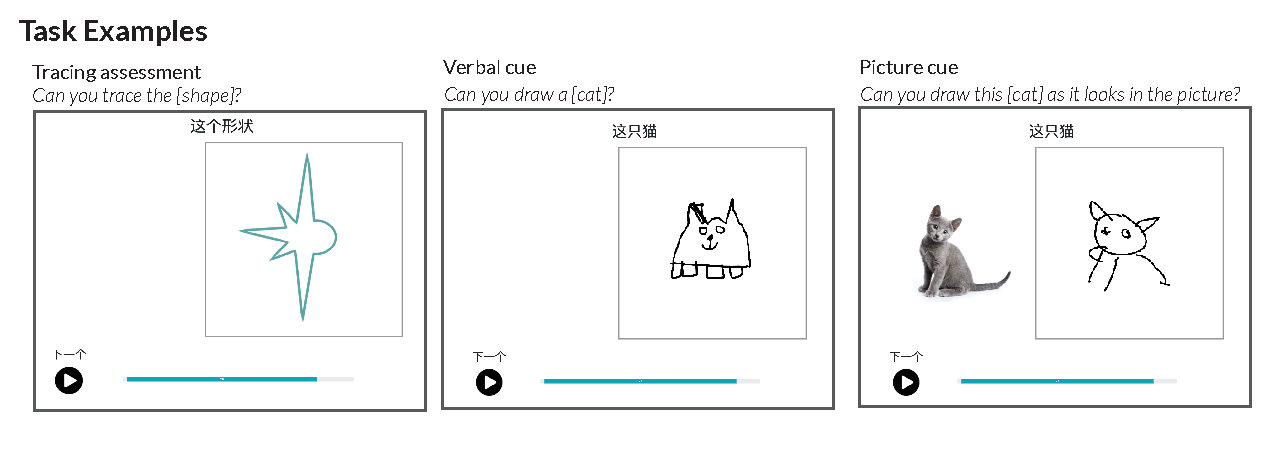
\includegraphics[width=1\linewidth]{figs/task_examples} \caption{Example trials from the tracing assessment and two drawing tasks.}\label{fig:example-tasks}
\end{figure}

\hypertarget{measuring-drawing-effort-covariates}{%
\subsection{Measuring drawing effort covariates}\label{measuring-drawing-effort-covariates}}

We recorded both the final drawings and the location of each stroke in a digital format, allowing us to precisely measure several different variables that provided proxies for the amount of effort children invested in producing each drawing.
Specifically, we measured: (1) the amount of time spent (i.e., end time of last stroke --- start time of first stroke), (2) the number of individual strokes drawn, and (3) the amount of ``ink'' used (i.e., proportion of drawing canvas that was filled).

\hypertarget{measuring-tracing-accuracy}{%
\subsection{Measuring Tracing Accuracy}\label{measuring-tracing-accuracy}}

As in prior work (Long et al., 2021), we used a semi-automated procedure for evaluating how accurately each child performed the tracing task that was validated against empirical judgments of tracing quality. In brief, we decomposed tracing accuracy into two components: a shape error component and a spatial error component. Shape error reflects how closely the participant's tracing matched the contours of the target shape; the spatial error reflects how closely the location, size, and orientation of the participant's tracing matched the target shape. These two error components were computed automatically for each tracing and used to yield a ``tracing score'' for each tracing that mirrors adult human judgments of tracing quality (see Appendix for details).

\hypertarget{measuring-drawing-recognizability}{%
\subsection{Measuring drawing recognizability}\label{measuring-drawing-recognizability}}

\hypertarget{human-recognition-scores}{%
\subsubsection{Human recognition scores}\label{human-recognition-scores}}

We measured the recognizability of each drawing via an online recognition experiment.
Adult participants based in the U.S. were recruited via Prolific for a 15-minute experiment, compensated at \$14/hour, and asked to identify the category depicted in a random subset of approximately 140 drawings.
Each subset of drawings was balanced with respect to age, category, and site, and each drawing was shown to 10 participants.
Participants were shown these drawings in a random sequence and asked ``What does this look like?''
Participants selected their responses from the set of 12 categories and were encouraged to provide their best guess if they were unsure.
No participants were excluded from analysis for missing the catch trial, which was included to verify that participants could accurately describe their goal in this task.
We then computed a recognition score for each drawing, reflecting the proportion of participants who correctly identified the target category.

\hypertarget{automated-recognition-scores}{%
\subsubsection{Automated recognition scores}\label{automated-recognition-scores}}

We used a combination of deep convolutional neural network (CNN) features and logistic regression to obtain automated recognition scores, per our preregistered protocol.
To encode the high-level visual features of each drawing, we passed each drawing into VGG-19 (Simonyan \& Zisserman, 2014), a deep CNN architecture that had been pre-trained on Imagenet classification and implemented in PyTorch (Paszke et al., 2017).
We extracted the feature representation of this drawing in the second-to-last layer of this network (FC6).
Feature representations in this layer consist of flat 4096-dimensional vectors, to which we applied channel-wise normalization.
Next, we used these features to train a leave-one-out 12-way logistic classifier with L2 regularization (tolerance = .1, regularization = .1), and used this classifier to predict the category label for each drawing.
To ensure a balanced distribution of drawings appearing in the training set, we randomly undersampled such that there was an equal number of drawings for each combination of geographical site (San Jose, Beijing) and the 12 categories.
No additional metadata about the age of the child who produced each sketch was provided to the model.
This procedure was repeated for each drawing in the dataset, yielding a binary recognition score for each drawing.

\hypertarget{statistical-models}{%
\subsection{Statistical models}\label{statistical-models}}

To evaluate our main hypotheses, we fit generalized linear mixed-effects models to the human recognition scores to assess the factors that influenced the recognizability of the drawings that children produced. A first generalized linear mixed effect model was fit to the recognizability scores for each drawing, including fixed effects of children's age (in years), geographical site (San Jose vs.~Beijing), and drawing task (verbal cue vs.~picture cue) and the three-way interaction between these key variables. We initially planned to include random slopes for the effect of drawing task on each child (as this varied within-subjects), and random slopes for the effect the full three-way interactions between task, age, and site on each category. However, models with this random-effects structure failed to converge, and the reported models use the maximal random effects structure that did converge, which included random slopes for the two-way interaction between task and age on each category.

In a secondary analysis, we investigated the degree to which any of the above effects were mediated by children's tracing abilities or the amount of effort that children expended while drawings.
We fit the same model above with additional fixed-effects terms for each child's estimated tracing score (see Measuring Tracing Abilities), the time that child spent drawing (in seconds), the amount of ``ink'' used (i.e.~percentage of non-white pixels in the drawn image), and the number of strokes produced.
These additional predictors were first z-scored before being included in the model.
Finally, we also assessed the degree to which tracing ability development differed across geographical sites, where tracing scores were modeled as a function of age (in years), site, and their interaction, with the same random-effects structure as the first model.

This analysis plan was pre-registered at \url{https://osf.io/qymjr}. While we had initially planned to use automated recognition scores as our main dependent variable, following prior work (Long et al., 2021), we found that these automated recognition scores were only modestly correlated with human recognition scores (\(r\) = 0.40, \(t\) = 22.78, p \textless{} .001); furthermore, descriptive plots of the automated recognition scores revealed an overall difference between the two drawing tasks that was not evident in the human recognition data. To be conservative, we thus fit all of our models to the human recognition data but have made all model predictions available to facilitate future research.

\hypertarget{results}{%
\section{Results}\label{results}}

\hypertarget{confirmatory-analyses}{%
\subsubsection{Confirmatory Analyses}\label{confirmatory-analyses}}

We found steady changes in the recognizability of children's drawings as a function of age (Figure \ref{fig:main-results}), replicating prior work using the verbal-cue paradigm under less controlled settings (Long et al., 2021).
Moreover, we found that this age-related change did not depend on the drawing task children completed: Children's drawings were just as recognizable when they were cued with a photograph (``Draw this rabbit as it looks in the picture'') as when they were cued with the category label (``Can you draw a rabbit?'').\\
While we thought that older children might produce more recognizable drawings when cued with a photograph of a highly prototypical exemplar, as adult participants do (Yang \& Fan, 2021), we did not find evidence of an interaction between age and cue type.
However, we did observe a main effect of geographical site: children in Beijing, China produced drawings that were more recognizable than did children in San Jose, USA (Table 1), reflecting steeper age-related gains earlier in development.

To follow up on this effect of site, we tested two potential sources of variation: visuomotor control and effort.
Insofar as differences in visuomotor control could explain differences between groups, we reasoned that this would manifest as a difference in tracing ability that predicts variation in drawing recognizability.
Instead, we found that children across the two sites were indistinguishable with respect to tracing ability on average (Figure \ref{fig:tracing}), although individual tracing scores were strong predictors of the recognizability of their own drawings, as in prior work (Long et al., 2021).
Next, we evaluated whether there were systematic differences in effort between the two groups, as measured by the amount of time each child spent producing their drawings and the number of strokes drawn.
Figure \ref{fig:effort-covariates} shows three effort covariates -- average intensity, number of strokes used, and time spent drawing -- measured for each drawing as a function of children's age, drawing task, and geographical site.\\
We found that children spent more time drawing when prompted with a picture cue than a verbal cue, and that children in the Beijing group spent more time on their drawings than their counterparts in San Jose.

We then included children's average tracing scores and effort covariates measured for each drawing (average intensity, number of strokes used, and time spent drawing) as fixed effects into a second generalized linear mixed-effects model (see Statistical Models).
If effort and/or tracing ability is sufficient to account for the differences between sites, we reasoned that we should no longer observe a main effect of geographical site on drawing recognizability in this expanded statistical model.
Instead, we observed a significant effect of geographical site (see Table 2), even after having accounted for the effect of individual differences in tracing ability as well as effort covariates for each drawing that was produced. Nonetheless, children's tracing abilities were clearly related to the degree they were able to produce recognizable drawings. Together, these results suggest that these site differences in the ability to produce recognizable drawings are not explained by differences in effort or tracing ability.

\hypertarget{exploratory-analyses}{%
\subsubsection{Exploratory Analyses}\label{exploratory-analyses}}

In a set of exploratory analyses, we examined how the developmental trajectory for drawing recognizability varied across object categories. For example, some object categories (e.g., cat) may be easier to draw than others (e.g., watch), resulting in shallower or steeper changes in recognizability over age. However, we did not have strong hypotheses about how these trajectories might additionally vary with geographical locations.

Figure \ref{fig:item-effects} shows considerable variation in drawing recognizability across the 12 categories as a function of geographical site and age. For example, certain distinctions between similar categories (e.g., cats and rabbits) were more difficult to make, especially for younger children. In addition, children in the Beijing group produced more recognizable drawings of certain categories at all ages -- including airplanes, birds, and rabbits -- while older children in San Jose produced more recognizable drawings of bikes. Figure \ref{fig:example-drawings} shows recognizable, randomly sampled example drawings from 6-year-olds at each category, site, and condition. As a whole, these exploratory analyses provide converging evidence for systematic differences between object categories and geographical site that are not easily attributable to differences in effort.

\begin{figure}[H]

{\centering \includegraphics[width=\textwidth]{figs/main-results-1} 

}

\caption{Proportion of drawings recognized as a function of the age of the child who completed each drawing, the geographical site they were tested at (San Jose vs. Beijing), and the type of drawing task they completed. Individual data points represent drawings within each condition by an individual participant and are slightly jittered. Error bars show bootstrapped 95 percent cofnidence intervals.}\label{fig:main-results}
\end{figure}

\begin{table}[ht]
\centering
\begin{tabular}{rrrrr}
  \hline
 & Estimate & Std. Error & z value & Pr($>$$|$z$|$) \\ 
  \hline
Intercept & 1.39 & 0.16 & 8.51 & 0.000 \\ 
  Task & 0.02 & 0.26 & 0.08 & 0.936 \\ 
  Age & 1.16 & 0.14 & 8.59 & 0.000 \\ 
  Site & 0.60 & 0.16 & 3.71 & 0.000 \\ 
  Task*Age & -0.14 & 0.19 & -0.73 & 0.467 \\ 
  Task*Site & -0.19 & 0.16 & -1.17 & 0.244 \\ 
  Age*Site & 0.15 & 0.16 & 0.91 & 0.361 \\ 
  Task*Age*Site & 0.06 & 0.16 & 0.38 & 0.706 \\ 
   \hline
\end{tabular}
\caption{Model coefficients from a generalized linear mixed mode predicting the recognizability of each drawing for the main experimental contrasts.} 
\end{table}

\begin{table}[ht]
\centering
\begin{tabular}{rrrrr}
  \hline
 & Estimate & Std. Error & z value & Pr($>$$|$z$|$) \\ 
  \hline
Intercept & 1.34 & 0.15 & 8.68 & 0.000 \\ 
  Task & -0.04 & 0.26 & -0.16 & 0.873 \\ 
  Age & 0.97 & 0.14 & 7.05 & 0.000 \\ 24
  Site & 0.80 & 0.16 & 5.04 & 0.000 \\ 
  Est. tracing score & 0.35 & 0.07 & 4.82 & 0.000 \\ 
  Avg. intensity & 0.06 & 0.02 & 2.47 & 0.013 \\ 
  Draw duration & -0.25 & 0.03 & -7.58 & 0.000 \\ 
  Number of strokes & 0.33 & 0.03 & 10.99 & 0.000 \\ 
  Task*Age & -0.17 & 0.19 & -0.90 & 0.370 \\ 
  Task*Site & -0.22 & 0.16 & -1.38 & 0.168 \\ 
  Age*Site & 0.04 & 0.16 & 0.22 & 0.823 \\ 
  Task*Age*Site & 0.07 & 0.16 & 0.43 & 0.665 \\ 
   \hline
\end{tabular}
\caption{Model coefficients from a generalized linear mixed mode predicting the recognizability of each drawing as a function the both the main experimental contrasts (task, site, and age) as well as several effort covariates and individual's estimates tracing abilities.} 
\end{table}

\begin{figure}[H]

{\centering \includegraphics[width=\textwidth]{figs/effort-covariates-1} 

}

\caption{Effort covariates measured during the drawing task -- amount of time spent drawing, amount of 'ink' used, and number of strokes used -- as function of the age of the child who completed each drawing, the geographical site they were tested at (San Jose vs. Beijing), and the type of drawing task they completed. Error bars show bootstrapped 95 percent cofnidence intervals.}\label{fig:effort-covariates}
\end{figure}

\begin{figure}[H]

{\centering \includegraphics[width=\textwidth]{figs/tracing-1} 

}

\caption{Average tracing scores across age and site; each dot represents an average tracing score obtained for each participant and are slightly jittered. Error bars represent bootstrapped 95 percent confidence intervals.}\label{fig:tracing}
\end{figure}

\begin{figure}[H]
\includegraphics[width=1\linewidth]{figs/example_drawings} \caption{Randomly sampled, highly recognized drawings for each task, category, and geographical site made by 6-year-old children.}\label{fig:example-drawings}
\end{figure}

\begin{figure}[H]

{\centering \includegraphics[width=\textwidth]{figs/item-effects-1} 

}

\caption{Developmental trajectory of drawing recognizability for each category and for each geographical site. Error bars represent 95 percent bootstrapped confidence intervals.}\label{fig:item-effects}
\end{figure}

\hypertarget{general-discussion}{%
\section{General Discussion}\label{general-discussion}}

Here we examined developmental change in children's ability to produce recognizable drawings of familiar visual concepts, and the degree to which this ability is constrained by retrieval of diagnostic attributes from memory.
We manipulated memory demands by either cueing children with a category label (``Can you draw a {[}cat{]}?'') or a color photo (``Can you draw this {[}cat{]} as it looks in the picture?''), and measured the recognizability of each drawing to adult observers.
To evaluate the generality of our findings, we recruited two groups of children in different sites: San Jose, USA and Beijing, China.
We found steady improvement from 4-9 years of age in both groups of children, replicating prior work conducted in a field setting (Long et al., 2021). We did not find an effect of drawing cue type, however, suggesting that younger children's drawings are unlikely to be constrained by their ability to recall category-diagnostic visual features when they are trying to draw them.

We also discovered that drawing recognizability differed between sites: children in the Beijing group produced more recognizable drawings than those in the San Jose group. While these group-level differences are intriguing, they remain consistent with wide variety of potential explanations.One idea is that children in the Beijing group drew at their preschool and elementary schools, whereas children in the San Jose group drew in a room at a children's science museum; these two testing environments could have created motivational differences that affected how much effort children put into their drawings. However, contra a strong version of this account, we found that the substantial individual variation in basic shape tracing ability and effort (as assessed via ink, time, and strokes spent while drwaing) was insufficient to account for differences in drawing recognizability between groups.

A second possibility is that the children who are learning to produce the complex, visually-demanding characters in the Chinese language that have meaningful subparts C. McBride \& Wang (2015) may develop more sophisticated visuomotor skills that are recruited while drawing. For example, the skills necessary to generate, combine, and arrange multiple shape parts in specific locations may be well-practiced by children learning to produce Chinese characters, and not well captured by the relatively simple shape tracing assessment that we used. Future work that relates writing, tracing, and drawing abilities within individual children learning to write different languages will be useful for understanding the degree to children's writing and drawing abilities inform eachother more generally.

Finally, we also found that the groups differed with respect to which visual concepts were easier for children to convey in their drawings, perhaps reflecting different patterns of exposure to these concepts.
Indeed, another natural question for future work concerns the relationship between the kind of experience children have with these visual concepts and the way they produce drawings of them. For example, if some children are exposed to a wide variety of illustrations of some concepts but not others (e.g., in books or other media), they may also be able to produce more recognizable drawings of those concepts. Conversely, if some children spend more time drawing certain visual concepts but not others (e.g., in school or at home), they may also be better at recognizing graphical representations of them in other contexts, and perhaps explicitly identifying their diagnostic features. Prior work has found that older children not only produce more recognizable drawings of object categories, but also tend to be better at recognizing other children's drawings (Long et al., 2021), providing evidence that visual production and recognition abilities are related throughout childhood at the group level. However, further investigation will be necessary for understanding what kinds of experience are responsible for concurrent developmental changes in these two behaviors at the individual level.

Thus, further systematic measurement of drawing behavior across a wider variety of geographical, socioeconomic, and cultural contexts will be crucial for producing more robust and precise estimates of developmental variability, critical to strongly evaluate causal theories of such variation (Amir \& McAuliffe, 2020; Carstensen, Cao, Gao, \& Frank, 2021; Frank, Braginsky, Yurovsky, \& Marchman, 2021). On the other hand, without such datasets it can be tempting to draw unwarranted causal inferences about the impact of single demographic covariates, such as nationality (Kuwabara \& Smith, 2016; Winner, 1989). We have thus made our drawing dataset publicly available to contribute to this more cumulative effort and also to reduce barriers to investigation of other aspects of these drawings other than their recognizability, such as which visual features children prioritized in their drawings, the order in which they drew them, as well as variation in visual style (Gernhardt, Rübeling, \& Keller, 2015; Senzaki, Masuda, \& Nand, 2014).

Overall our result thus support a domain-specific account of the development of drawing abilities: children's ability to convey their knowledge about familiar visual concepts does not seem to be influenced by how they are cued to draw a given visual concept, and changes systematically across age in two different geographical contexts. We propose that further investigation into the factors that influence how children learn to identify and combine the relevant diagonstic features of different visual concepts will further explain individual and age-related variation in drawing abilities. More broadly, we believe that this approach to concurrently quantifying multiple sources of variation in the context of rich, naturalistic behaviors will lead to more robust and unified theories of cognitive development.

\hypertarget{acknowledgements}{%
\section{Acknowledgements}\label{acknowledgements}}

{[}BLINDED{]}

\hypertarget{references}{%
\section{References}\label{references}}

\begingroup
\setlength{\parindent}{-0.5in}
\setlength{\leftskip}{0.5in}

\endgroup

\hypertarget{refs}{}
\begin{CSLReferences}{1}{0}
\leavevmode\vadjust pre{\hypertarget{ref-amir2020cross}{}}%
Amir, D., \& McAuliffe, K. (2020). Cross-cultural, developmental psychology: Integrating approaches and key insights. \emph{Evolution and Human Behavior}, \emph{41}(5), 430--444.

\leavevmode\vadjust pre{\hypertarget{ref-barrett1976symbolism}{}}%
Barrett, M., \& Light, P. (1976). Symbolism and intellectual realism in children's drawings. \emph{British Journal of Educational Psychology}, \emph{46}(2), 198--202.

\leavevmode\vadjust pre{\hypertarget{ref-bloom1998intention}{}}%
Bloom, P., \& Markson, L. (1998). Intention and analogy in children's naming of pictorial representations. \emph{Psychological Science}, \emph{9}(3), 200--204.

\leavevmode\vadjust pre{\hypertarget{ref-bremmer1984prior}{}}%
Bremner, J. G., \& Moore, S. (1984). Prior visual inspection and object naming: Two factors that enhance hidden feature inclusion in young children's drawings. \emph{British Journal of Developmental Psychology}, \emph{2}(4), 371--376.

\leavevmode\vadjust pre{\hypertarget{ref-carstensen2021investigating}{}}%
Carstensen, A., Cao, A., Gao, S., \& Frank, M. C. (2021). Investigating cross-cultural differences in reasoning, vision, and social cognition through replication. \emph{Proceedings of the Annual Meeting of the Cognitive Science Society}, \emph{43}.

\leavevmode\vadjust pre{\hypertarget{ref-cohn2012explaining}{}}%
Cohn, N. (2012). Explaining {``i can't draw''}: Parallels between the structure and development of language and drawing. \emph{Human Development}, \emph{55}(4), 167--192.

\leavevmode\vadjust pre{\hypertarget{ref-dekker2011dorsal}{}}%
Dekker, T., Mareschal, D., Sereno, M. I., \& Johnson, M. H. (2011). Dorsal and ventral stream activation and object recognition performance in school-age children. \emph{NeuroImage}, \emph{57}(3), 659--670.

\leavevmode\vadjust pre{\hypertarget{ref-fan2018common}{}}%
Fan, J. E., Yamins, D. L., \& Turk-Browne, N. B. (2018). Common object representations for visual production and recognition. \emph{Cognitive Science}, \emph{42}(8), 2670--2698.

\leavevmode\vadjust pre{\hypertarget{ref-frank2021variability}{}}%
Frank, M. C., Braginsky, M., Yurovsky, D., \& Marchman, V. A. (2021). \emph{Variability and consistency in early language learning: The wordbank project}. MIT Press.

\leavevmode\vadjust pre{\hypertarget{ref-freeman1987current}{}}%
Freeman, N. H. (1987). Current problems in the development of representational picture-production. \emph{Archives de Psychologie}.

\leavevmode\vadjust pre{\hypertarget{ref-fury1997children}{}}%
Fury, G., Carlson, E. A., \& Sroufe, A. (1997). Children's representations of attachment relationships in family drawings. \emph{Child Development}, \emph{68}(6), 1154--1164.

\leavevmode\vadjust pre{\hypertarget{ref-gernhardt2015cultural}{}}%
Gernhardt, A., Rübeling, H., \& Keller, H. (2015). Cultural perspectives on children's tadpole drawings: At the interface between representation and production. \emph{Frontiers in Psychology}, \emph{6}, 812.

\leavevmode\vadjust pre{\hypertarget{ref-hoffmann2018u}{}}%
Hoffmann, D. L., Standish, C. D., Garcia-Diez, M., Pettitt, P. B., Milton, J., Zilhão, J., \ldots{} others. (2018). U-th dating of carbonate crusts reveals neandertal origin of iberian cave art. \emph{Science}, \emph{359}(6378), 912--915.

\leavevmode\vadjust pre{\hypertarget{ref-huntsinger2011cultural}{}}%
Huntsinger, C. S., Jose, P. E., Krieg, D. B., \& Luo, Z. (2011). Cultural differences in chinese american and european american children's drawing skills over time. \emph{Early Childhood Research Quarterly}, \emph{26}(1), 134--145.

\leavevmode\vadjust pre{\hypertarget{ref-karmiloff1990constraints}{}}%
Karmiloff-Smith, A. (1990). Constraints on representational change: Evidence from children's drawing. \emph{Cognition}, \emph{34}(1), 57--83.

\leavevmode\vadjust pre{\hypertarget{ref-kellogg1969analyzing}{}}%
Kellogg, R. (1969). \emph{Analyzing children's art}. National Press Books Palo Alto, CA.

\leavevmode\vadjust pre{\hypertarget{ref-kuwabara2016cultural}{}}%
Kuwabara, M., \& Smith, L. B. (2016). Cultural differences in visual object recognition in 3-year-old children. \emph{Journal of Experimental Child Psychology}, \emph{147}, 22--38.

\leavevmode\vadjust pre{\hypertarget{ref-la2001children}{}}%
La Voy, S. K., Pedersen, W. C., Reitz, J. M., Brauch, A. A., Luxenberg, T. M., \& Nofsinger, C. C. (2001). Children's drawings: A cross-cultural analysis from japan and the united states. \emph{School Psychology International}, \emph{22}(1), 53--63.

\leavevmode\vadjust pre{\hypertarget{ref-light1983effects}{}}%
Light, P., \& Simmons, B. (1983). The effects of a communication task upon the representation of depth relationships in young children's drawings. \emph{Journal of Experimental Child Psychology}, \emph{35}(1), 81--92.

\leavevmode\vadjust pre{\hypertarget{ref-long2021parallel}{}}%
Long, B., Fan, J., Chai, Z., \& Frank, M. C. (2021). \emph{Parallel developmental changes in children's drawing and recognition of visual concepts}.

\leavevmode\vadjust pre{\hypertarget{ref-long2018drawings}{}}%
Long, B., Fan, J., \& Frank, M. C. (2018). Drawings as a window into developmental changes in object representations. \emph{Proceedings of the 40th Annual Meeting of the Cognitive Science Society}.

\leavevmode\vadjust pre{\hypertarget{ref-luquet1927dessin}{}}%
Luquet, G.-H. (1927). \emph{Le dessin enfantin.(biblioth{è}que de psychologie de l" enfant et de p{é}dagogie.).}

\leavevmode\vadjust pre{\hypertarget{ref-mcbride2016chinese}{}}%
McBride, C. A. (2016). Is chinese special? Four aspects of chinese literacy acquisition that might distinguish learning chinese from learning alphabetic orthographies. \emph{Educational Psychology Review}, \emph{28}(3), 523--549.

\leavevmode\vadjust pre{\hypertarget{ref-mcbride2015learning}{}}%
McBride, C., \& Wang, Y. (2015). Learning to read chinese: Universal and unique cognitive cores. \emph{Child Development Perspectives}, \emph{9}(3), 196--200.

\leavevmode\vadjust pre{\hypertarget{ref-minsky1972artificial}{}}%
Minsky, M., \& Papert, S. (1972). \emph{Artificial intelligence progress report}. Cambridge, MA, USA: Massachusetts Institute of Technology.

\leavevmode\vadjust pre{\hypertarget{ref-natu2016development}{}}%
Natu, V. S., Barnett, M. A., Hartley, J., Gomez, J., Stigliani, A., \& Grill-Spector, K. (2016). Development of neural sensitivity to face identity correlates with perceptual discriminability. \emph{Journal of Neuroscience}, \emph{36}(42), 10893--10907.

\leavevmode\vadjust pre{\hypertarget{ref-pailian2016visual}{}}%
Pailian, H., Libertus, M. E., Feigenson, L., \& Halberda, J. (2016). Visual working memory capacity increases between ages 3 and 8 years, controlling for gains in attention, perception, and executive control. \emph{Attention, Perception, \& Psychophysics}, \emph{78}(6), 1556--1573.

\leavevmode\vadjust pre{\hypertarget{ref-paszke2017automatic}{}}%
Paszke, A., Gross, S., Chintala, S., Chanan, G., Yang, E., DeVito, Z., \ldots{} Lerer, A. (2017). \emph{Automatic differentiation in PyTorch}.

\leavevmode\vadjust pre{\hypertarget{ref-piaget1929child}{}}%
Piaget, J. (1929). The child's concept of the world. \emph{Londres, Routldge \& Kegan Paul}.

\leavevmode\vadjust pre{\hypertarget{ref-rehrig2018does}{}}%
Rehrig, G., \& Stromswold, K. (2018). What does the DAP: IQ measure?: Drawing comparisons between drawing performance and developmental assessments. \emph{The Journal of Genetic Psychology}, \emph{179}(1), 9--18.

\leavevmode\vadjust pre{\hypertarget{ref-senzaki2014holistic}{}}%
Senzaki, S., Masuda, T., \& Nand, K. (2014). Holistic versus analytic expressions in artworks: Cross-cultural differences and similarities in drawings and collages by canadian and japanese school-age children. \emph{Journal of Cross-Cultural Psychology}, \emph{45}(8), 1297--1316.

\leavevmode\vadjust pre{\hypertarget{ref-simonyan2014very}{}}%
Simonyan, K., \& Zisserman, A. (2014). Very deep convolutional networks for large-scale image recognition. \emph{arXiv Preprint arXiv:1409.1556}.

\leavevmode\vadjust pre{\hypertarget{ref-sitton1992drawing}{}}%
Sitton, R., \& Light, P. (1992). Drawing to differentiate: Flexibility in young children's human figure drawings. \emph{British Journal of Developmental Psychology}, \emph{10}(1), 25--33.

\leavevmode\vadjust pre{\hypertarget{ref-willats2006making}{}}%
Willats, J. (2006). \emph{Making sense of children's drawings}. Psychology Press.

\leavevmode\vadjust pre{\hypertarget{ref-winner1989can}{}}%
Winner, E. (1989). How can chinese children draw so well? \emph{Journal of Aesthetic Education}, \emph{23}(1), 41--63.

\leavevmode\vadjust pre{\hypertarget{ref-yang2021visual}{}}%
Yang, J., \& Fan, J. E. (2021). Visual communication of object concepts at different levels of abstraction. \emph{arXiv Preprint arXiv:2106.02775}.

\end{CSLReferences}


\end{document}
